% !TEX root = main.tex
\chapter{Simulation}
\label{chap:simulations}


\section{Star-CCM+}
  Star-CCM+ was used to run the simulations of the wing first in the windtunnel for verification. As meshing and running the simulations were heavy computational tasks, the computations were run on the \emph{Niflheim Linux cluster supercomputer}, which is installed at the Department of Physics at DTU.

  The program numerically solves the Navier-Stokes equations, which are derived by the conservation of energy, mass and momentum through a volumetric flow. As Star-CCM+ uses the finite volume method, the equations are discretized to the conservative form: The in- and outgoing flux through a control volume must be conserved. Mathematically, this is expressed as:

  \begin{align}
    \frac{\delta}{\delta t} \iiint Q dV + \iint F dA = 0
  \end{align}
  Where $Q$ is the vector of the conserved variables (eg. $\rho =$ density), $F$ is the vector of fluxes(eg. $\rho u =$ mass flux, $\rho u^2 + p=$ momentum flux + pressure force) and $V$ is the control volume element and $A$is the surface area of the control volume element. The turbulence model Star-CCM+ employs is a K-epsilon turbulence model which is the most commonly used in computational fluid dynamics. %The equations Star-CCM+ solves are the turbulent kinetic energy $k$:
  %\begin{align}
  %  \frac{\delta (\rho k)}{\delta t} + \frac{\delta (\rho k u_i)}{\delta x_i} &= \frac{\delta}{\delta x_j} \left(\frac{\mu_t}{\sigma_k}\frac{\delta k)}{\delta x_j}\right) + 2\mu_t E_{ij}E_{ij}-\rho \epsilon
  %  \intertext{and the dissipation $\epsilon$:}
  %  \frac{\delta (\rho \epsilon)}{\delta t} + \frac{\delta (\rho \epsilon u_i)}{\delta x_i} &= \frac{\delta}{\delta x_j} \left(\frac{\mu_t}{\sigma_\epsilon}\frac{\delta \epsilon)}{\delta x_j}\right) + C_{1\epsilon} \frac{\epsilon}{k} 2\mu_t E_{ij}E_{ij}-C_{2\epsilon}\rho \frac{\epsilon^2}{k}
  %\end{align}

  The interested reader of how Star-CCM+ works is referred to the \emph{User Guide Star-CCM+, version 13.02}.

\section{Mesh Generation}
\label{sec:mesh}
  The mesh has to be structured in accordance to best practice. Areas with high velocity and pressure gradiants have to be dissolved in acceptable resolutions, in order to ensure correct results. Running an initial test on a generic mesh made it clear where the volumemesh requires greater resolution. Gradiants are easily visible around the wing's leading edge, and generally around the solid bodies. Furthermore, aligning the mesh with the flow improves accuracy and rate of convergence. To determine the convergence of simulation results six different mesh resolutions where used to examine the simulations for the windtunnel setup with a wind velocity of $\SI{40}{\metre\per\second}$. Finding the minimum mesh resolution where results have converged with higer resolution results, means a minimum computation time can be achived and thereby allowing for more simulations to be run.

  \begin{figure}
    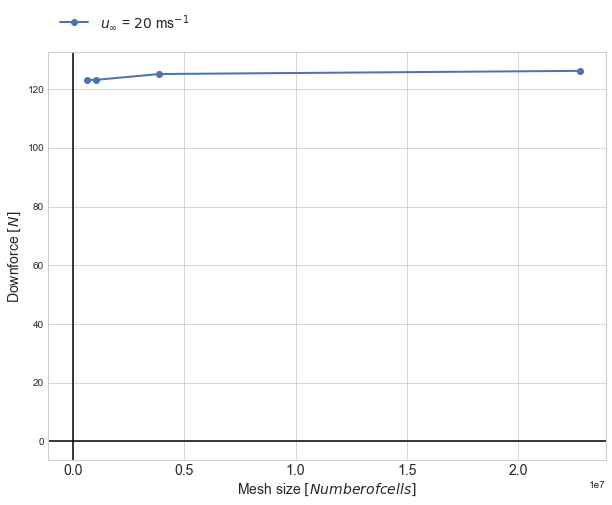
\includegraphics[width=\textwidth]{DFprmeshsize}
    \caption{Normalized downforce as a function of mesh size. Plotted to see the convergence towards the same force.}
    \label{fig:DFprmeshsize}
  \end{figure}

  Generating a mesh of correct size is done by sampling downforce over a range of mesh sizes. In figure \ref{fig:DFprmeshsize}, the normalized downforce is plotted as a function of the mesh size. The mesh independence study shows that the function converges to acceptable levels near the mesh size $\SI{.4E7}{}$, and serves to be a good compromise between results and computing time.

  \section{Verification of Simulation Results}
  \label{sec:simulationcomparison}


  \begin{figure}
    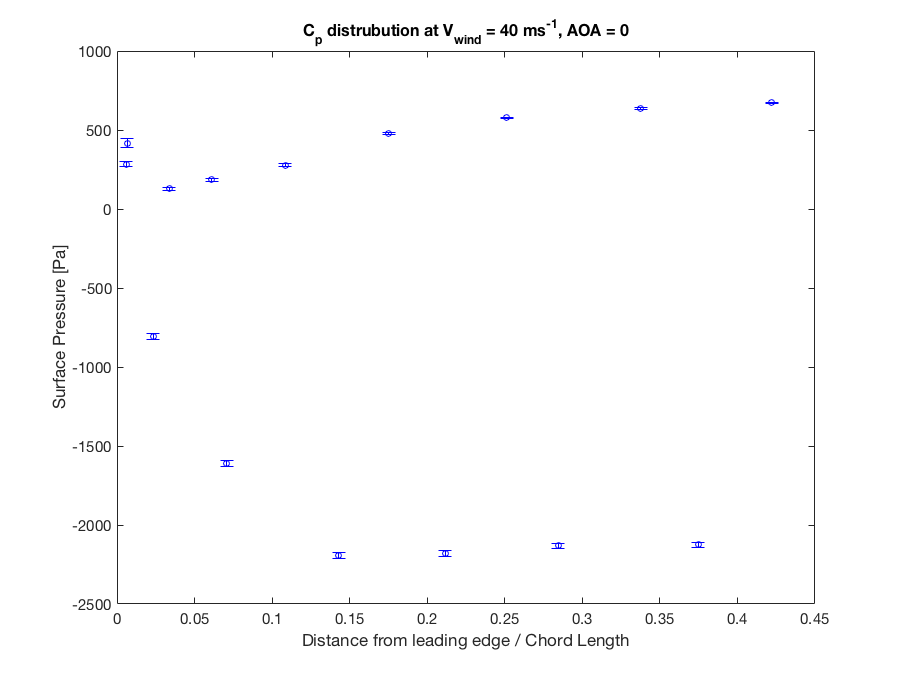
\includegraphics[width=\textwidth]{surfacepressureint}
    \label{fig:surfacepressureint}
  \end{figure}


  \begin{figure}
    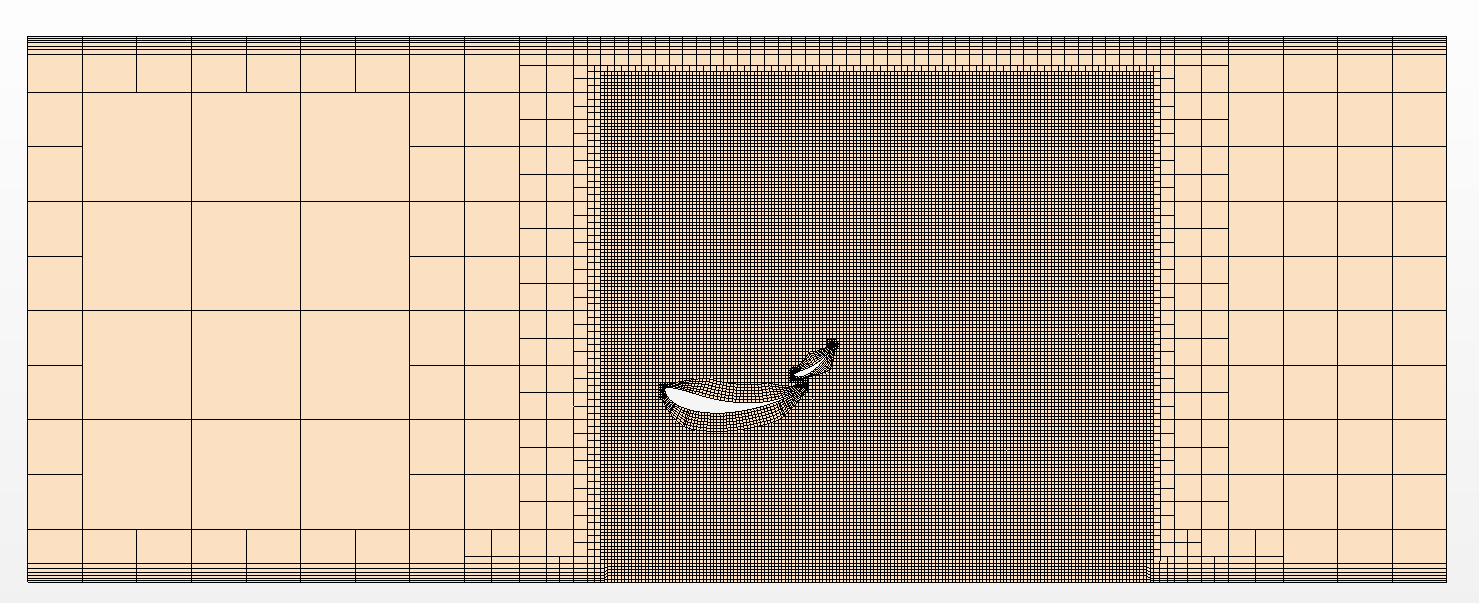
\includegraphics[width=\textwidth]{mesh3point8millcells}
    \label{fig:mesh3point8mill}
  \end{figure}


  \begin{figure}
    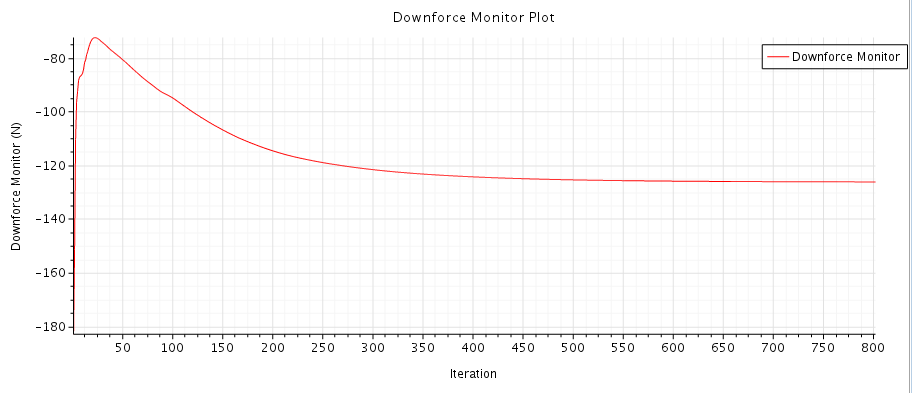
\includegraphics[width=\textwidth]{downforcemonitor}
    \caption{Monitor of the convergence of the downforce over the number of iterations in Star-CCM+, here shown for a wind velocity of $\SI{40}{\metre\per\second}$.}
    \label{fig:downforcemonitor}
  \end{figure}

  \begin{figure}
    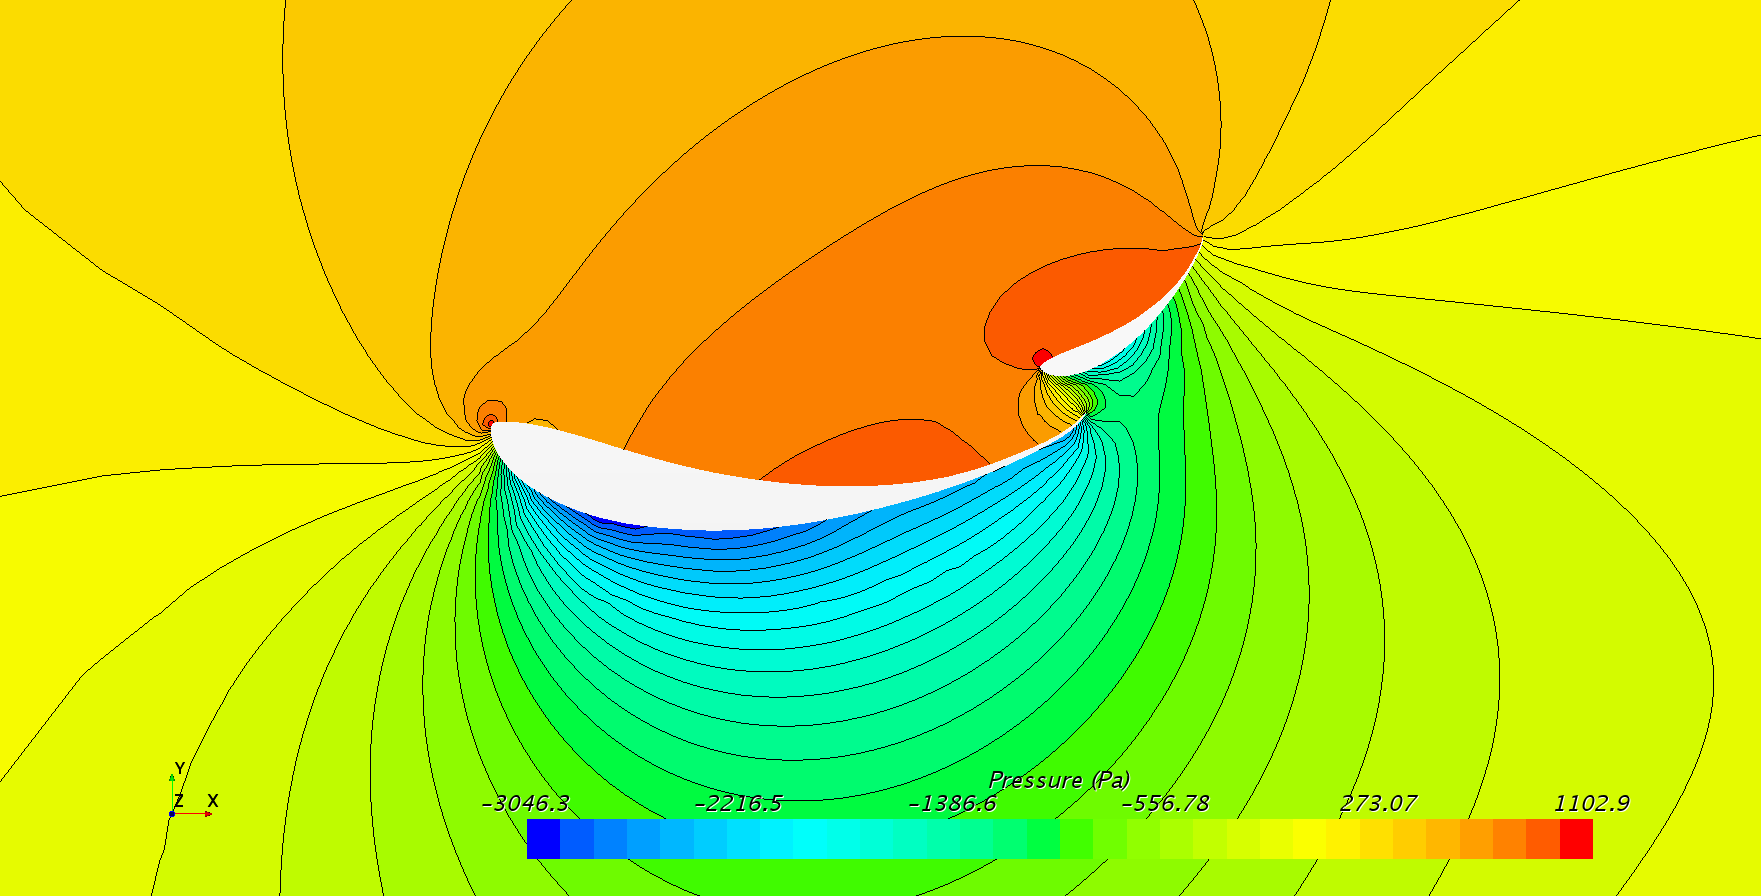
\includegraphics[width=\textwidth]{pressureScalarV40}
    \caption{Scalar view of the pressure distribution surrounding the two elements of the wing, here at a wind velocity of $\SI{40}{\metre\per\second}$.}
    \label{fig:pressureScalarV40}
  \end{figure}

  \begin{figure}
    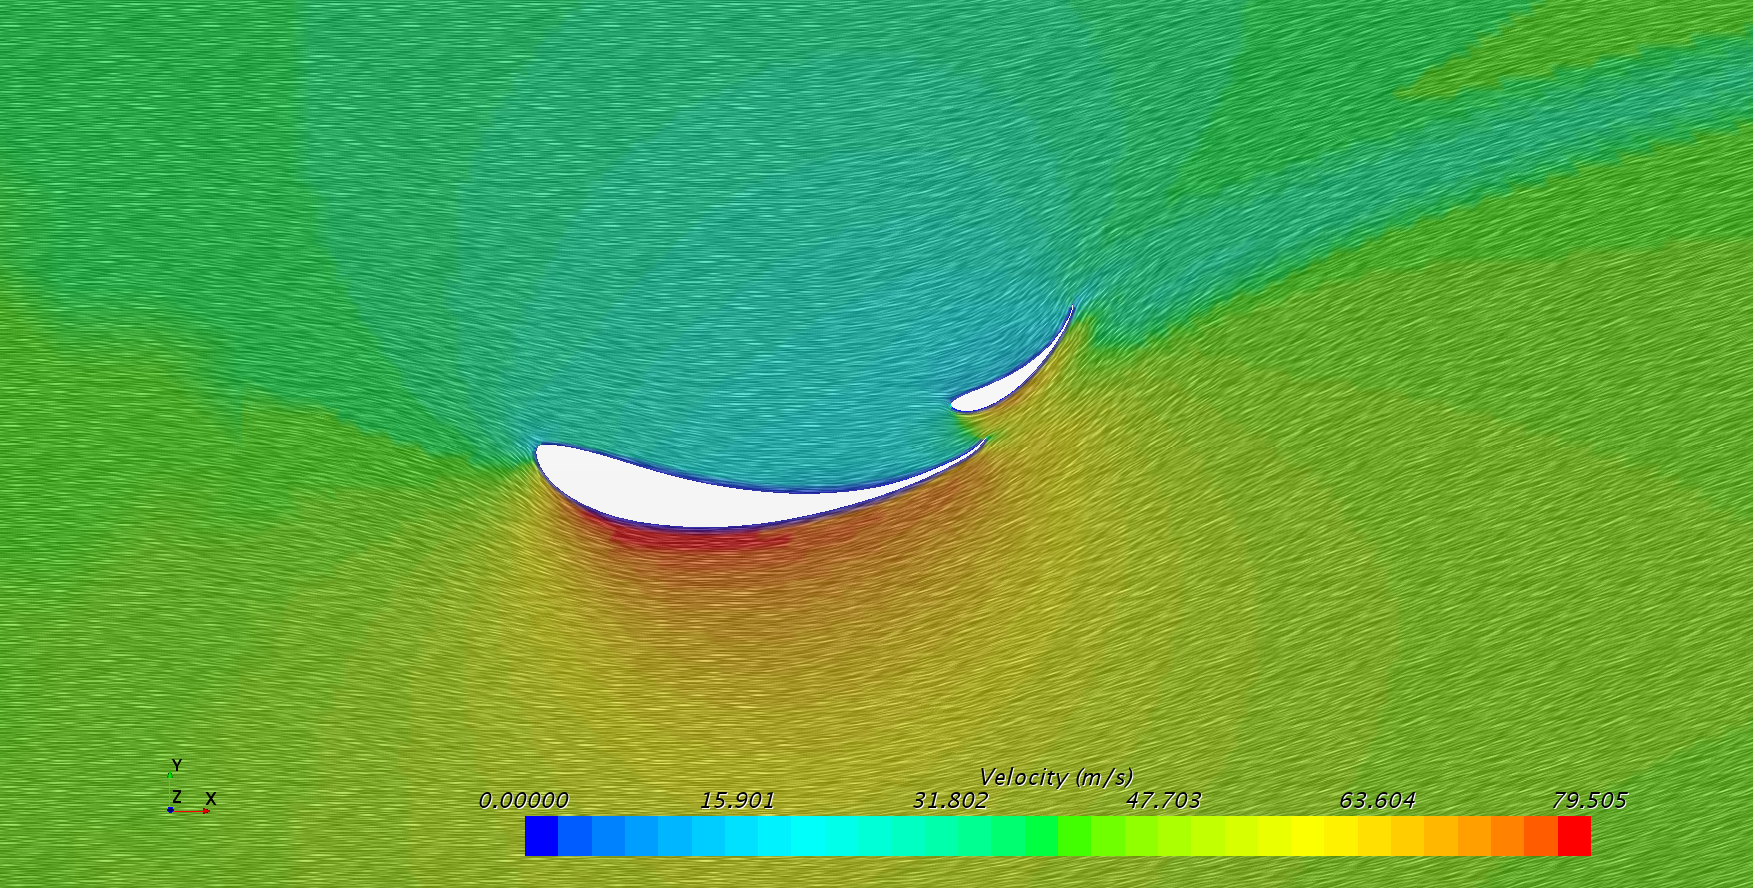
\includegraphics[width=\textwidth]{velocityScalarV40}
    \caption{Vector view of the wind velocity surrounding the wing, here at a wind velocity of $\SI{40}{\metre\per\second}$.}
    \label{fig:velocityScalarV40}
  \end{figure}

  From the simulations the surface pressure of the airfoils was also found, and saved to compare with the measurements of the surface pressure from the real wind tunnel test. The simulated surface pressure is shown in figure \ref{fig:simsurfacepressurev40}.

  \begin{figure}
    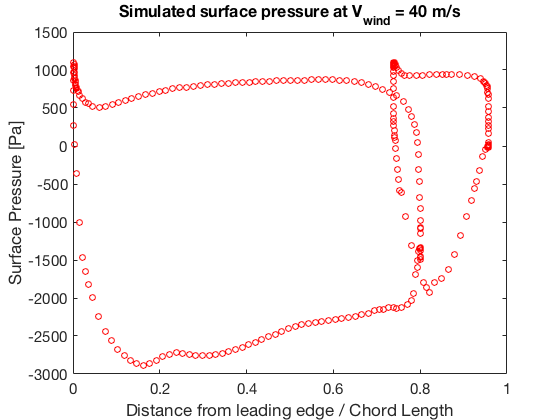
\includegraphics[width=\textwidth]{simsurfacepressurev40}
    \caption{Simulated surface pressure on both elements of the wing. To the left the larger element surface pressure and the smaller elements surface pressure is shown right. Simulated at wind velocity of $\SI{40}{\metre\per\second}$.}
    \label{fig:simsurfacepressurev40}
  \end{figure}



  \begin{align}
    C_p \equiv \frac{p-p_{\infty}}{\frac{1}{2}\rho_{\infty}V_{\infty}^2},
  \end{align}



  \begin{figure}
    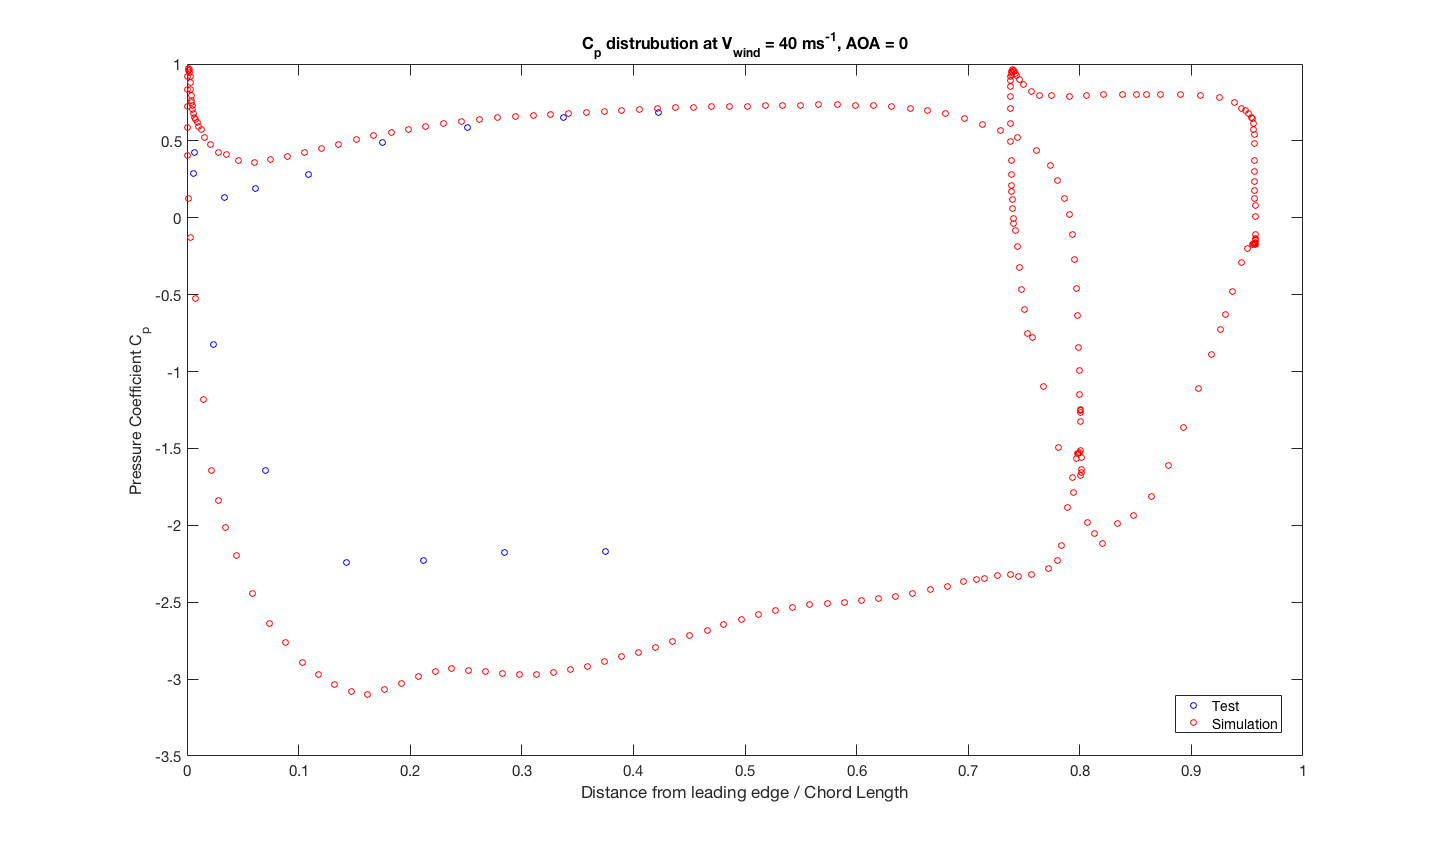
\includegraphics[width=\textwidth]{CpV40}
    \caption{Comparison of simulated and test found $C_p$ values at a wind velocity of $\SI{40}{\metre\per\second}$.}
    \label{fig:CpV40}
  \end{figure}

  The use of simulations for designing an aerodynamic package for the race car for the moment is usefull as a way to insure the realtive pressure distrubtion aorund the wing is as wanted, and ensuring that the flow does not seperate at unwanted locations. However further work on the correlation between simulated downforce and measured downforce is still needed and the work will continue with the Vermilion Racing team, in order to have the best possibilities to design a good aero-package before having to build it.

  Lastly worth noting is when the simulated flow is visualized by streamlines, the vortex generation at the rear of the wing, as mentioned in section \ref{subsec:endplates}, is shown clearly in figure \ref{fig:simvortex}. It is clear that the size of the produced vortices are interacting with the side walls of the wind tunnel. A sugestion for further testing of an wing with such large vortex generation would be to use a wind tunnel with a larger cross-secton to avoid interactions with the side walls.

  \begin{figure}
    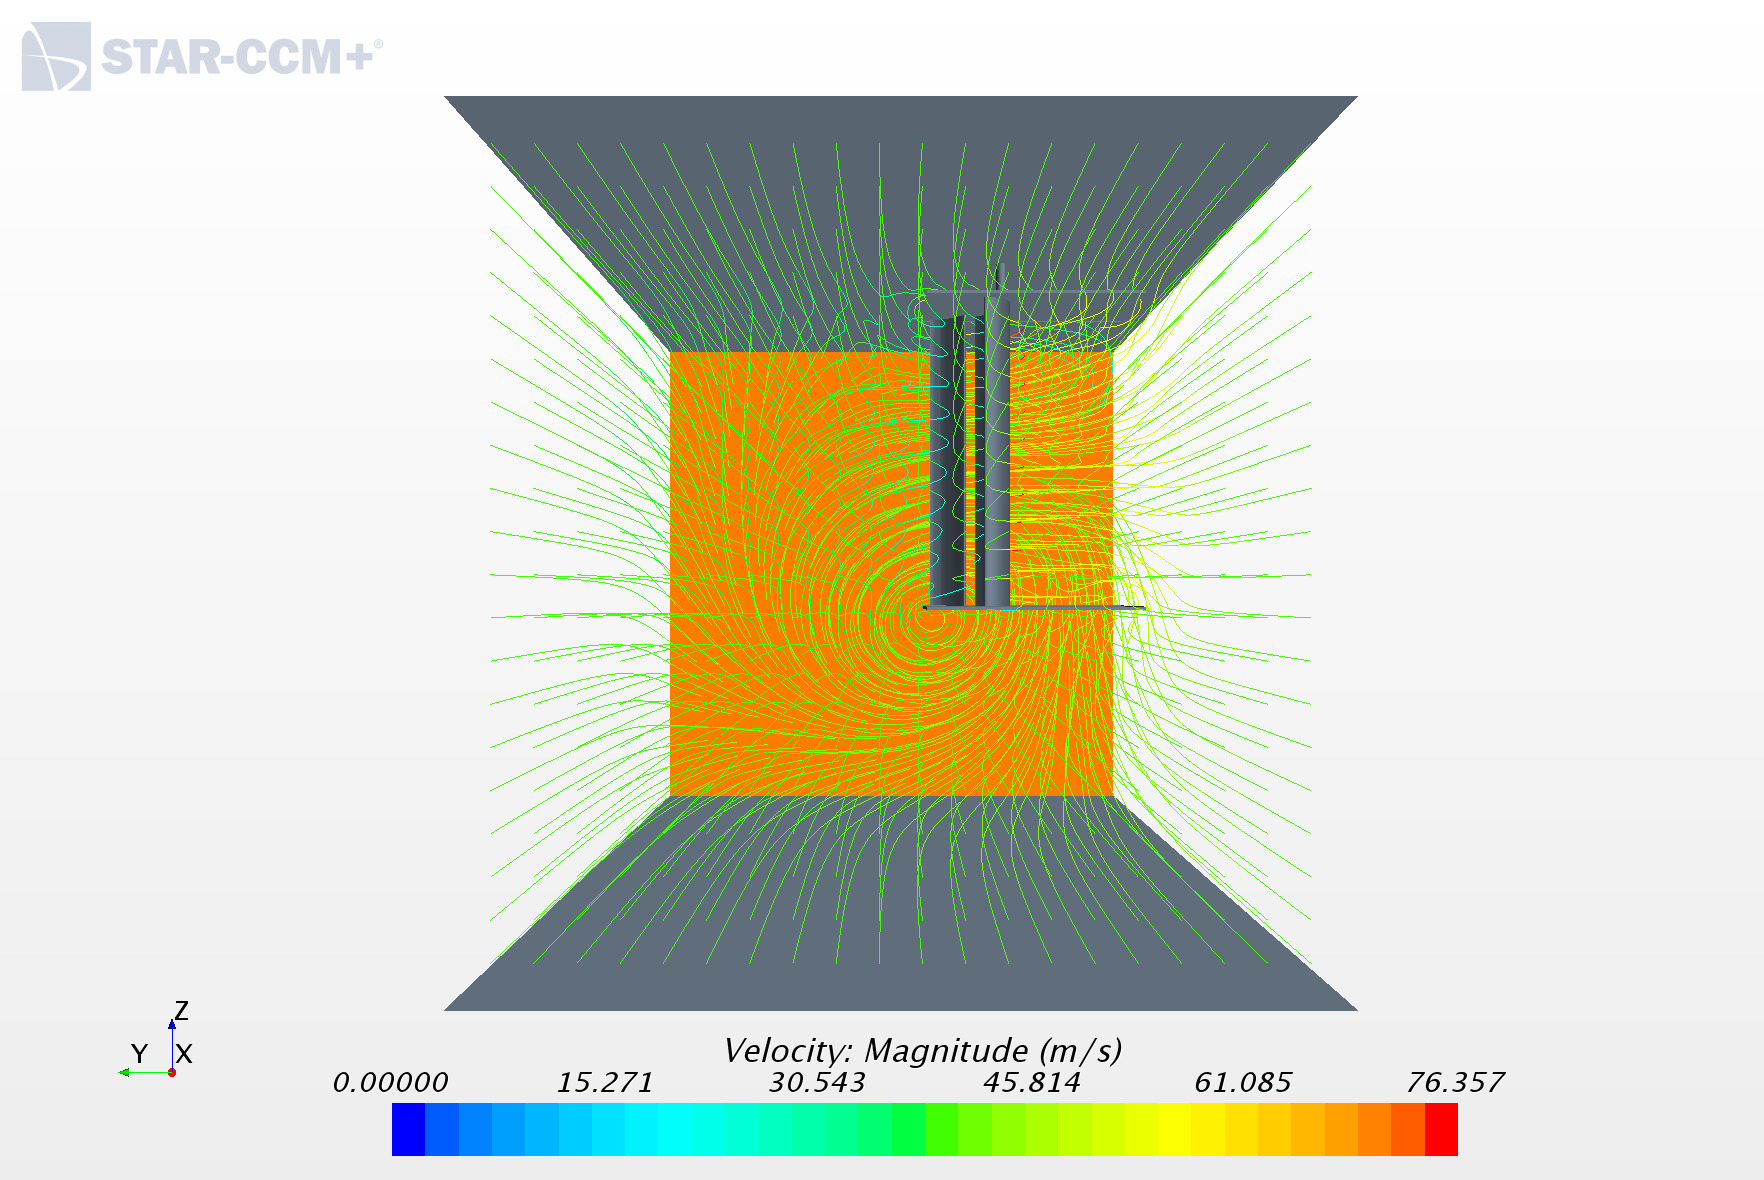
\includegraphics[width=\textwidth]{simulatedvortex}
    \caption{Visualization by streamlines of the simulated airflow around the wing. Vortex generation at the rear of the wing is visiable.}
    \label{fig:simvortex}
  \end{figure}

  \subsection{Multi-Element Wing Optimization}
  The influence of the two wing elements relative position on lift was examined to optimize the downforce the rear wing provides to the car at a given velocity. This relative position optimization was performed in the software package \emph{MultiElements Airfoils} provided from \emph{Hanley Innovations}. A scatterplot of the relative position is seen in figure \ref{fig:multieleoptimization}. The trailing edge of the first element is seem as the dark lines, and the position of the second elements leading edge is plotted, where the resulting lift coefficient is embedded as color. The redder the better lift coefficient. After sweeping, a maximum lift of $C_L = 2.60$  at $u = \SI{15}{\metre\per\second}$. is found with the leading edge of the secondary element placed at $x=\SI{0.5}{\metre},y=\SI{-0.01}{\metre}$ relative to the leading edge of the main element.

  \begin{figure}
    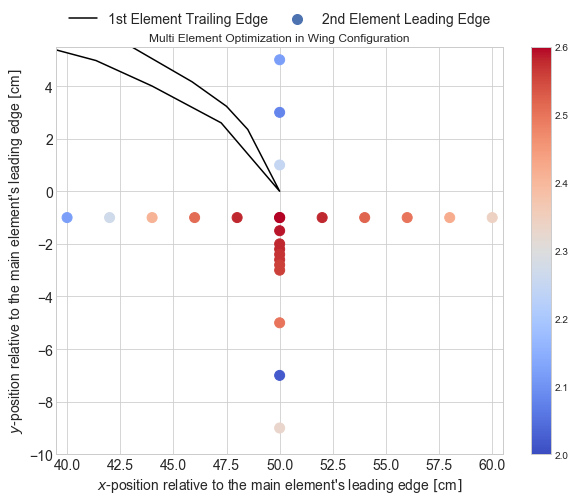
\includegraphics[width=\textwidth]{multieleoptimization2}
    \caption{Optimization of the two element wing. The redder the dots, the higher the lift coefficient.}
    \label{fig:multieleoptimization}
  \end{figure}

\section{Downforce Estimate of Full Scale Wing}
\fixme{Maybe save for defense}
